\documentclass[12pt, a4paper, titlepage]{article}
\usepackage[utf8]{inputenc}
\usepackage{indentfirst}
\usepackage{polski}
\usepackage{array}
\usepackage{graphicx}
\usepackage{listings}
\usepackage{color}
\lstset{language=C,caption={Descriptive Caption Text},label=DescriptiveLabel}

\begin{document}
    \input{./00_strona_tytulowa}
    \tableofcontents
    \section {Opis projektu}
Celem projektu było utworzenie systemu pozwalającego prowadzącemu zajęcia monitorować komputery w~pracowni laboratoryjnej. Aplikacja do pracy wymaga skonfigurowania serwera aplikacji (IIS z~obsługą ASP.NET), połączonego siecią lokalną z~komputerami w~laboratorium. 

Serwer udostępnia serwis internetowy, do którego prowadzący zajęcia loguje się za pomocą przeglądarki internetowej. Udostępnia on podgląd pulpitów i~informacji o~procesach uruchomionych na aktywnych stanowiskach komputerowych. W~domyślnym widoku dostępny jest podgląd ekranów z~wybranej pracowni, każdy w oddzielnej komórce siatki -- podobnie jak w~systemach monitoringu wizyjnego CCTV. Po wybraniu odpowiedniego stanowiska, program wyświetla podgląd z~pulpitu danego komputera w wyższej jakości wraz z~dodatkowymi danymi. Są to uruchomione aplikacje oraz otwarte karty w~przeglądarkach komputerowych. W~czasie, gdy prowadzący będzie zalogowany na swój panel, aplikacje klienckie zbierają dane i~przesyłają je na serwer. Monitoring nie odbywa się w momencie, gdy żaden prowadzący nie prowadzi monitoringu -- oszczędność zasobów sprzętowych oraz przepustowości sieci lokalnej.

System umożliwia definiowane tzw. ,,czarnej listy'' procesów, a~w~momencie wykrycia, że użytkownik uruchomił jakikolwiek proces z~tej listy, zapisuje we właściwej tabeli informacje o~naruszeniach. Dodatkowo, do każdego naruszenia zapisywany jest zrzut ekranu.

    \subsection {Wybór tematu}
Temat został wybrany posługując się dwoma kryteriami: potencjalnej przydatności oraz poziomu umiejętności grupy projektowej. Wybrany projekt może być podstawą dla aplikacji do kompleksowego zbierania danych o~pracy pracowników w~miejscu pracy lub monitoringu publicznie dostępnych komputerów.

Przykładem takiego powszechnie wykorzystywanego systemu jest system podglądu kas samoobsługowych w~supermarketach. Udostępniane klientom jest zwykle kilka kas, będących pod ciągłym nadzorem pracownika sklepu, który oprócz rozwiązywania problemów i~pomocy klientom, jest odpowiedzialny także za sprawdzanie, czy produkty są odpowiednio skanowane.

Należy wspomnieć o aspekcie prawnym stosowania takich aplikacji. Zgodnie z~polskim prawem monitoring musi szanować godność oraz dobra osobiste pracownika (art. 11 Kodeksu Pracy).

    \subsection{Architektura}

W~tym rozdziale krótko przedstawiono architekturę projektowanego systemu. W~dalszej części niniejszej dokumentacji będzie to punkt odniesienia do sposobu działania aplikacji.

\begin{figure} [!ht]
    \centering
    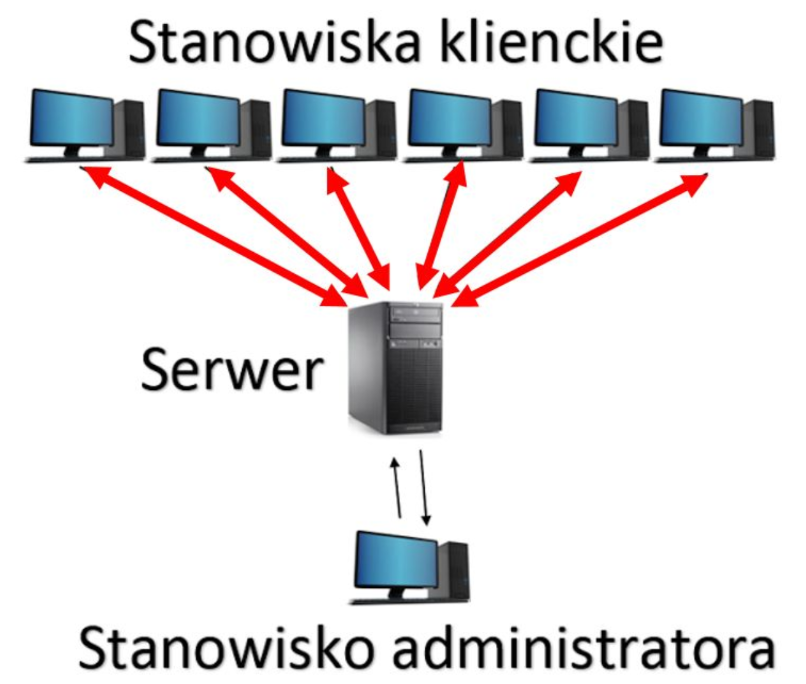
\includegraphics[height=8cm,width=10cm]{architektura}
    \caption{Projekt architektury systemu}
    \label{fig:architektura}
\end{figure}

Rysunek \ref{fig:architektura}. przedstawia architekturę projektowanego systemu. Stanowiska klienckie to komputery użytkowników np. w~sali komputerowej, na których uruchamiane są aplikacje klienckie. Stanowisko administratora, jest to komputer, który potrzebuje dostępu do przeglądarki internetowej, aby skorzystać z~aplikacji. Serwer natomiast udostępnia serwis internetowy, do którego łączą się administratorzy/nauczyciele i~stanowiska kliencie. Tutaj znajduje się także baza danych systemu.
    \section {Wymagania funkcjonalne}
W poniższej sekcji przedstawiono wymagania funkcjonalne projektowanego systemu -- zbiór funkcjonalności, które zestaw aplikacji powinien spełnić. Wymagania dotyczą danych obszarów działania oraz związane są z aktorami (zewnętrzny obiekt wchodzący w interakcję z systemem).

Na początku przedstawiono aktorów. Ich lista wraz z~opisem znajdują się w~Tabeli \ref{tab:actors}.

\begin{table}[!ht]
\caption{Aktorzy systemu}
\label{tab:actors}
\begin{tabular}{| m{2,7cm} | m{11cm} |} \hline
Aktor & Opis aktora \\ \hline
Aplikacja agenta   & Program zainstalowany na stanowisku                        komputerowym. Zbiera dane z maszyny klienta.\\ \hline

Użytkownik zalogowany  & Jest to użytkownik, który ma możliwość                              zalogowania się na stronie, która znajduje się na                         serwerze i umożliwia podgląd\\
                       
                        & stanowisk połączonych z serwerem. \\ \hline

Administrator   & Jest to użytkownik zalogowany, ale oprócz jego \\                                      &funkcjonalności może także zarządzać klientami, grupami \\
                &stanowisk oraz użytkownikami. \\ \hline

\end{tabular}
\end{table}

\newpage

Tabela \ref{tab:functionalreq}. przedstawia zebrane wymagania funkcjonalne projektowanego systemu. W~kolejnych kolumnach opisano żądaną funkcjonalność, aktora (lub aktorów) (według Tabeli \ref{tab:actors}) uczestniczącego w~danej funkcjonalności oraz obszar działania tożsamy z~modułami aplikacji.

\begin{table}[!ht]
\caption{Lista wymagań funkcjonalnych}
\label{tab:functionalreq}
\begin{tabular}{| m{0.5cm} | m{7cm} | m{3cm} | m{2cm} |}
\hline
l.p. 
    & Funkcjonalność 
    & Aktor 
    & Obszar 
\\ \hline
    1.   
    & Wykonywanie zrzutów ekranu w~określonej częstotliwości i~przesyłanie ich do serwera
    & Aplikacja agenta
    & Agent, Serwer
\\ \hline
    2. 
    & Definiowanie stanowisk komputerowych w systemie.
    & Administrator
    & Serwis internetowy
\\ \hline
    3.
    & Tworzenie i zarządzanie grupami stanowisk.
    & Administrator
    & Serwis internetowy
\\ \hline
    4. 
    & Podgląd wielu stanowisk jednocześnie w ramach wybranej grupy.
    & Administrator, Użytkownik zalogowany
    & Serwis internetowy
\\ \hline
    5. 
    & Podgląd obrazu w lepszej jakości ze stanowisk wraz z listą uruchomionych aplikacji oraz kart z przeglądarek internetowych
    & Administrator, Użytkownik zalogowany
    & Serwis internetowy
\\ \hline
    6.
    & Zarządzanie czarną listy procesów, które umożliwią alarmowanie monitorującego o naruszeniu zasad.
    & Administrator
    & Serwis internetowy
\\ \hline
    7.
    & Wysyłanie wiadomości tekstowej do wybranego komputera lub grupy stanowisk.
    & Administrator, Użytkownik zalogowany
    & Serwis internetowy
\\ \hline
    8.
    & Zarządzanie użytkownikami i administratorami.
    & Administrator
    & Serwis internetowy
\\ \hline
    9.
    & Zarządzanie uprawnieniami użytkowników do sal.
    & Administrator
    & Serwis internetowy
\\ \hline
    
\end{tabular}
\end{table}



    \section{Wymagania pozafunkcjonalne}
W tej sekcji zostały przedstawione kryteria i~ograniczenia, jakie są nałożone na system. Ze względu na architekturę zaprezentowaną w sekcji 1.2, wymagania zostały rozdzielone na trzy kategorie: aplikację klienta, serwera systemu oraz aplikacji webowej. Poniższe wymagania są niezbędne do poprawnego działania wszystkich aplikacji.

\vspace{1.0cm}

Dla aplikacji klienta:
\begin{itemize}
    \item System operacyjny Windows 7 lub nowszy
    \item minimalna wersja .NET Framework 4.5.2
    \item aplikacja okienkowa uruchamiana wraz ze startem systemu
    \item polska wersja językowa
\end{itemize}

\vspace{0.5cm}

Dla serwera systemu:
\begin{itemize}
    \item System operacyjny Windows Server 2012 (ew. Windows 8) lub nowszy
    \item minimalna wersja .NET Framework 4.5.2
    \item minimalna wersja Entity Framework 6.1
    \item Microsoft SQL Server 2016
    \item serwer IIS z zainstalowaną obsługą ASP.NET
\end{itemize}

\vspace{0.5cm}

Dla aplikacji webowej:
\begin{itemize}
    \item przeglądarka internetowa (minimalne wersje: Google Chrome 56, Mozilla Firefox 52 lub Opera 43)
    \item aplikacja dostępna wyłącznie w języku polskim
\end{itemize}
    \section{Środowisko i użyte technologie}
Wykonanie projektu zakłada wykorzystanie kilku narzędzi, bibliotek, edytorów oraz środowiska programistycznego. Odpowiednią listę przedstawiono poniżej.

\begin{itemize}
    \item Microsoft Visual Studio 2015 (IDE),
    \item język programowania: C\#,
    \item Microsoft SQL Server 2016 (baza danych),
    \item Microsoft SQL Server Management Studio (zarządzanie bazą danych),
    \item .NET Framework 4.5.2,
    \item Entity Framework 6.1 (ORM),
    \item ASP.NET MVC 4.6,
    \item serwis GitHub (repozytorium kodu źródłowego),
    \item narzędzie sharelatex.com (sporządzenie niniejszej dokumentacji),
    \item biblioteka SignalR.
\end{itemize}
    \section{Projekt bazy danych}
Poniższy rozdział zawiera projekt bazy danych systemu. Będzie ona przechowywała informacje o użytkownikach, grupach laboratoryjnych, stanowiskach komputerowych oraz uprawnieniach użytkowników do sal. 

Rysunek \ref{fig:diag_rel} przedstawia diagram relacyjny projektowanej bazy danych. Opis poszczególnych pól oraz ich znaczeń opisano w Tabelach \ref{tab:user_descr} (User), \ref{tab:comp_descr} (Computer), \ref{tab:classroom_descr} (Classroom), \ref{tab:croomperm_descr} (ClassroomPermission), \ref{tab:blacklist_descr} (Blacklist) oraz \ref{tab:abuse_descr} (Abuse).

\begin{figure} [!ht]
    \centering
    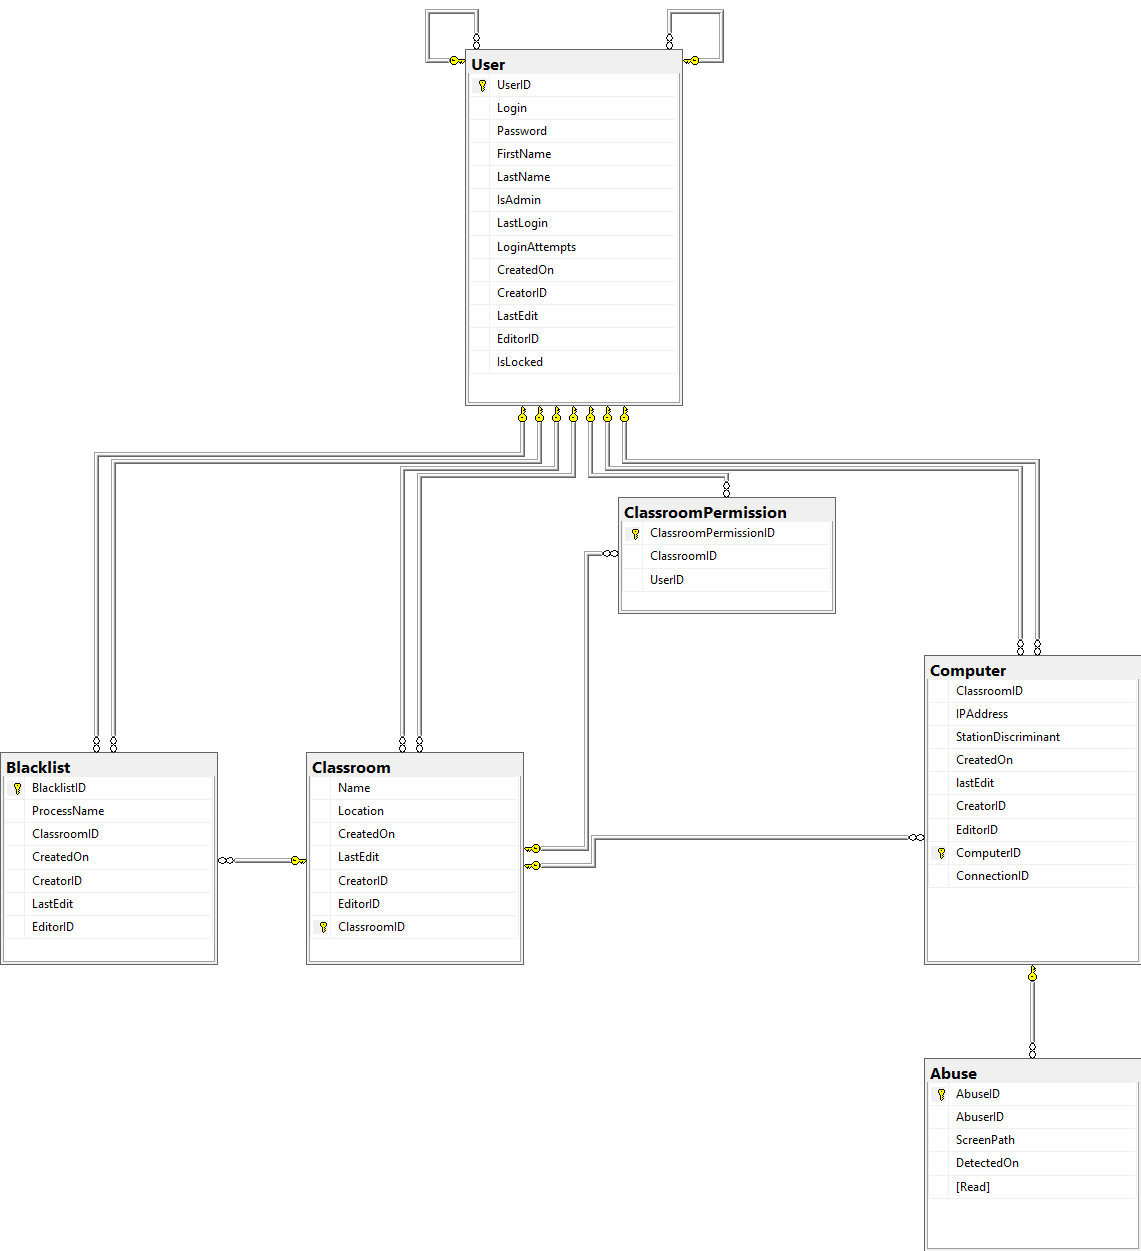
\includegraphics[height=12cm,width=15cm]{diagram_relacyjny}
    \caption{Diagram relacyjny bazy danych}
    \label{fig:diag_rel}
\end{figure}



\begin{table}[!ht]
\caption{Opis kolumn w tabeli User}
\label{tab:user_descr}
\begin{tabular}{| m{3.5cm} | m{10.5cm} |} 

\hline
Pole & Opis \\ \hline

UserID & unikatowy identyfikator użytkownika\\ \hline
Login & krótki ciąg znaków używany przez użytkowników do logowania \\ \hline 
Password & hasło do konta \\ \hline
FirstName & imię użytkownika \\ \hline
LastName & nazwisko użytkownika \\ \hline
IsAdmin & pole logiczne, którego wartość ,,Prawda'' określa, że użytkownik jest administratorem \\ \hline
LastLogin & data ostatniego poprawnego logowania do serwisu \\ \hline
LoginAttempts & licznik błędnych prób logowania \\ \hline
CreatedOn & data utworzenia użytkownika \\ \hline
CreatorID & identyfikator użytkownika, który utworzył to konto \\ \hline
LastEdit & data ostatniej edycji danych tego użytkownika \\ \hline
EditorID & identyfikator użytkownika, który ostatnio edytował dane tego konta \\ \hline
IsLocked & pole logiczne określające, czy użytkownik jest zablokowany. Gdy wartością jest prawda, użytkownik nie może się zalogować do systemu.
\\ \hline
\end{tabular}
\end{table}

\begin{table}[!ht]
\caption{Opis kolumn w tabeli Computer}
\label{tab:comp_descr}
\begin{tabular}{| m{3.5cm} | m{10.5cm} |} 

\hline
Pole & Opis \\ \hline

ID & identyfikator komputera \\ \hline
IPAdress & adres IP komputera \\ \hline
StationDiscriminant & krótki tekstowy wyróżnik\\ \hline
CreatedOn & data utworzenia tego stanowiska \\ \hline
LastEdit & data ostatniej modyfikacji danych stanowiska \\ \hline
CreatorID & identyfikator administratora, który utworzył to stanowisko \\ \hline
EditorID & identyfikator administratora, który ostatnio edytował dane tego stanowiska \\ \hline
IsConnected & oznacza, czy dany komputer jest aktualnie podłączony do serwera \\ \hline
\end{tabular}
\end{table}

\begin{table}[!ht]
\caption{\label{tab:classroom_descr}Opis kolumn w tabeli Classroom}
\begin{tabular}{| m{3.5cm} | m{10.5cm} |} 

\hline
Pole & Opis\\ \hline

ClassroomID & identyfikator sali komputerowej \\ \hline
Name & nazwa sali komputerowej  (np. jej numer)\\ \hline
Location & opis miejsca, gdzie znajduje się sala (np. budynek, piętro) \\ \hline
CreatedOn & data utworzenia sali \\ \hline
LastEdit & data ostatniej modyfikacji danych sali \\ \hline
CreatorID & identyfikator administratora, który utworzył salę \\ \hline
EditorID & identyfikator administratora, który ostatnio edytował dane sali\\ \hline
\end{tabular}
\end{table}

\begin{table}[!ht]
\caption{\label{tab:croomperm_descr}Opis kolumn w tabeli ClassroomPermission}
\begin{tabular}{| m{3.5cm} | m{10.5cm} |} 

\hline
Pole & Opis\\ \hline

ClassroomPermID & identyfikator uprawnienia do edycji danych sali \\ \hline
ClassroomID & identyfikator sali, której dotyczy to uprawnienie \\ \hline
UserID & identyfikator użytkownika, którego dotyczy to uprawnienie\\ \hline

\end{tabular}
\end{table}

\begin{table}[!ht]
\caption{\label{tab:blacklist_descr}Opis kolumn w tabeli Blacklist}
\begin{tabular}{| m{3.5cm} | m{10.5cm} |} 

\hline
Pole & Opis\\ \hline

BlacklistID & identyfikator pozycji czarnej listy \\ \hline
ProcessName & nazwa procesu niedozwolonego \\ \hline
ClassroomID & identyfikator sali, której dotyczy ta pozycja \\ \hline
CreatedOn & data utworzenia \\ \hline
LastEdit & data ostatniej modyfikacji danych czarnej listy \\ \hline
CreatorID & identyfikator administratora, który utworzył pozycję czarnej listy \\ \hline
EditorID & identyfikator administratora, który ostatnio edytował dane pozycji\\ \hline

\end{tabular}
\end{table}

\begin{table}[!ht]
\caption{\label{tab:abuse_descr}Opis kolumn w tabeli Abuse}
\begin{tabular}{| m{3.5cm} | m{10.5cm} |} 

\hline
Pole & Opis\\ \hline

AbuseID & identyfikator naruszenia \\ \hline
AbuserID & identyfikator komputera, którego dotyczy to naruszenie \\ \hline
ScreenPath & nazwa pliku ze zrzutem ekranu wykrytego naruszenia \\ \hline
DetectedOn & data i godzina wykrycia naruszenia \\ \hline

\end{tabular}
\end{table}
    \section{Diagramy klas}

W poniższym rozdziale zaprezentowane zostały diagramy klas. Ukazano uproszczoną strukturę systemu ze względu na podział na klasy. Podstawowym kryterium podziału jest program, w którym znajdują się dane klasy. W pierwszej części przedstawiono klasy użyte w aplikacji klienta, w drugiej natomiast wykorzystane w serwisie internetowym.

\subsection {Aplikacja klienta}
Poniżej przedstawiono diagram klas znajdujących się w aplikacji klienta. Klasy ApplicationForm i Podglad są oknami Windows Form. Klasy ServerHandler oraz ServerConnection są wykorzystywane do połączenia z serwerem za pomocą biblioteki SignalR. Klasa Spy udostepnia za to metody odpowiedzialne za tworzenie zrzutu ekranu, pobieranie listy otwartych stron oraz aktywnych procesów.

\begin{figure} [!ht]
    \centering
    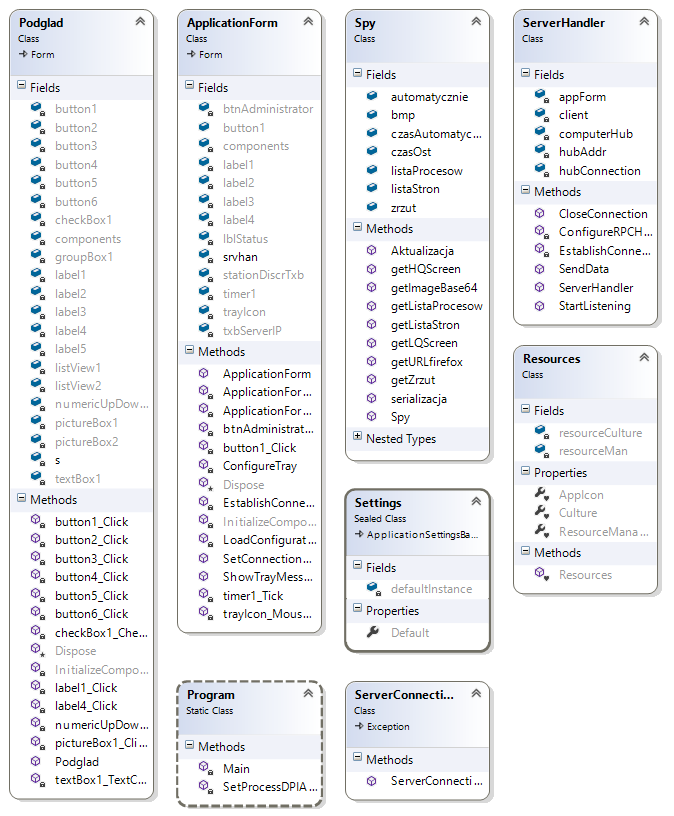
\includegraphics[height=10cm,width=9cm]{diagramklas_klient}
    \caption{Diagram klas - aplikacja klienta}
    \label{fig:my_label}
\end{figure}

\subsection{Serwer}

Poniżej natomiast znajdują się diagramy klas w aplikacji serwera. Zostały one podzielone na dwie części, ze względu na ilość klas, jaka została użyta. Klasy Computer, Classroom, ClassroomPermision oraz User zostały napisane do obsługi bazy danych zgodnie z metodą CodeFirst przy wykorzystaniu Entity Framework. Oprócz tego znajdują się kontrolery odpowiedzialne za każdy widok oraz same widoki. Dodatkowo są zaimplementowane huby potrzebne do połączenia z klientami.

\begin{figure} [!ht]
    \centering
    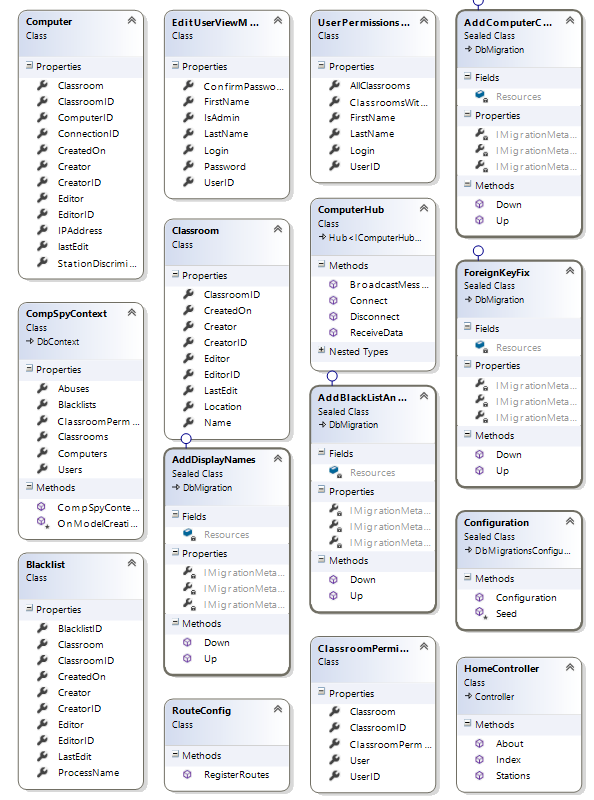
\includegraphics[height=12cm,width=12cm]{diagramklas_serwer1}
    \caption{Diagram klas - aplikacja serwera cz. 1}
    \label{fig:my_label}
\end{figure}
\newpage
W modelach oprócz tych klas związanych z bazą danych znajdują się jeszcze klasy Abuse i Blacklist. Natomiast jeśli chodzi o widoki, to zostały podzielone na kategorie: Account, Classrooms, Computers, Home, Shared, Suirvalance oraz User.

\begin{figure} [!ht]
    \centering
    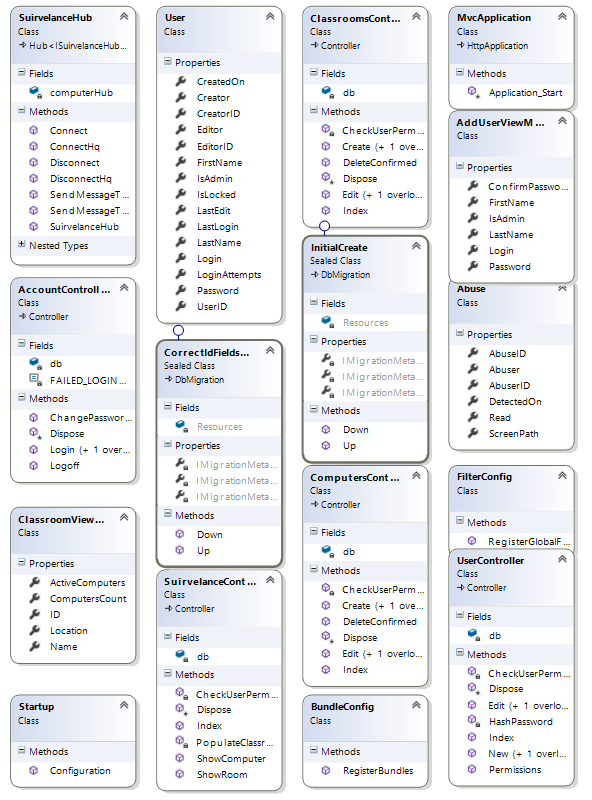
\includegraphics[height=12cm,width=12cm]{diagramklas_serwer2}
    \caption{Diagram klas - aplikacja serwera cz. 2}
    \label{fig:my_label}
\end{figure}
    \section{Diagram przypadków użycia}

Rozdział przedstawia diagram przypadków użycia projektowanego systemu sporządzony w języku UML. Wykorzystuje się go w celu zaprezentowania, jaką rolę mogą wykonywać poszczególni aktorzy w kontakcie z opisywanym systemem oraz przejrzyście prezentuje, w jaki sposób zachowuje się dany system i jak wygląda jego interakcja z użytkownikami w konkretnych sytuacjach.

\newline
\begin{figure} [!ht]
    \centering
    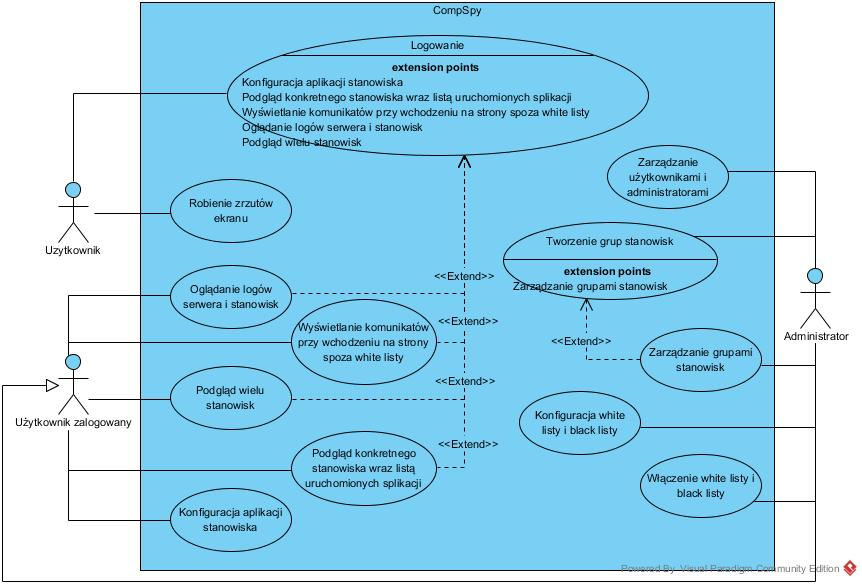
\includegraphics[height=12cm,width=15cm]{PT_UC_Diagram}
    \caption{Diagram przypadków użycia}
    \label{fig:my_label}
\end{figure}

    \section{Szkic interfejsu użytkownika}

Poniżej przedstawiony jest projekt interfejsu użytkownika. Pierwsza część przedstawia widoki w serwisie internetowym. Druga natomiast część przedstawia okno programu klienta na stanowisku klienckim. 

\subsection{Serwis internetowy}
Na poniższych rysunkach przedstawiono projekty poszczególnych widoków strony internetowej serwisu. Rysunek nr 8 przestawia projekt strony głównej, którą każdy zobaczy po wpisaniu adresu serwisu internetowego.
\begin{figure} [!ht]
    \centering
    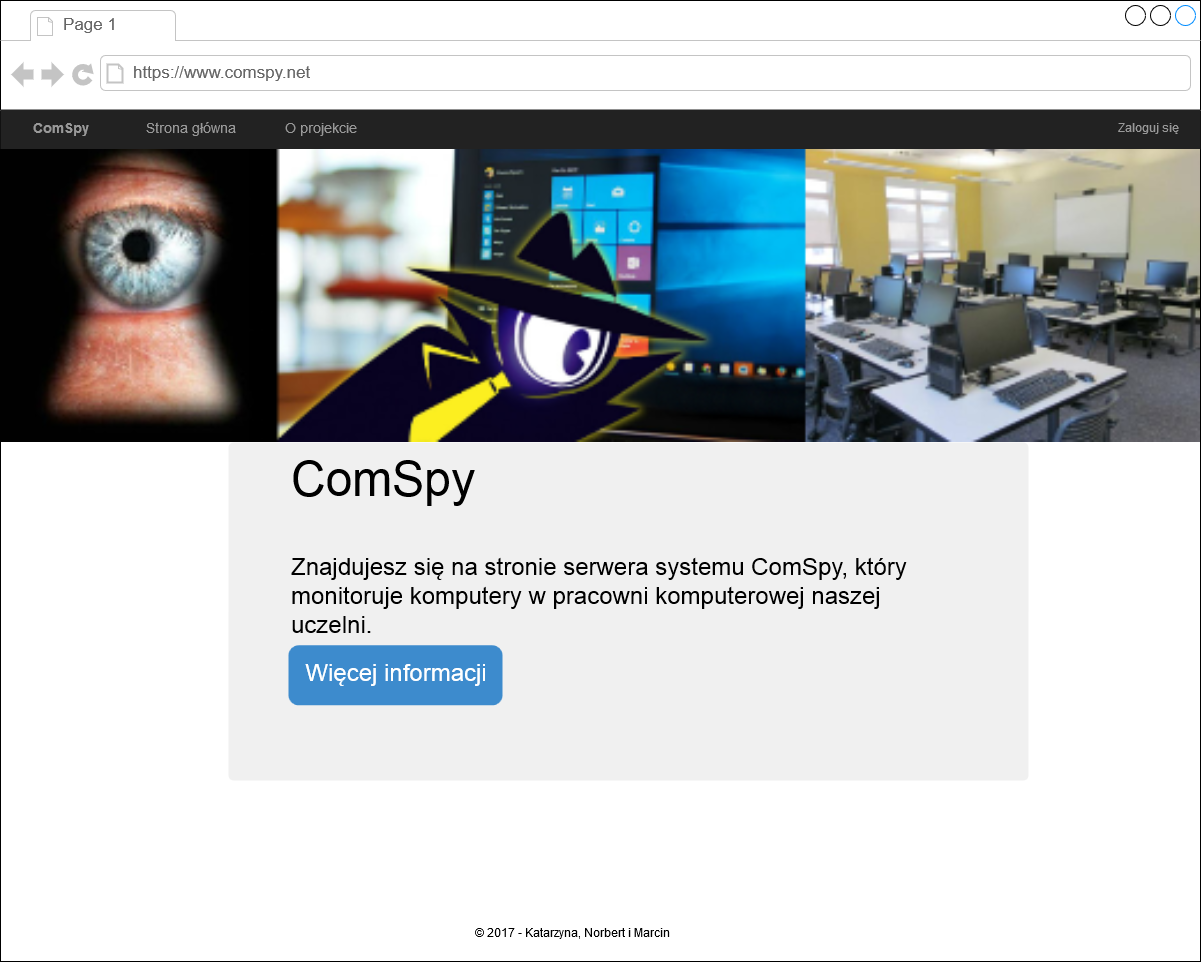
\includegraphics[height=12cm,width=15cm]{interfejs_homepage}
    \caption{Projekt strony głównej}
    \label{fig:my_label}
\end{figure}

\newpage
Rysunek nr 9 przedstawia panel logowania. W celu zalogowania się użytkownik jest proszony o podanie loginu i hasła. W przypadku wprowadzenia złych danych jest wyświetlany komunikat o błędzie i niepowodzeniu logowania.
\begin{figure} [!ht]
    \centering
    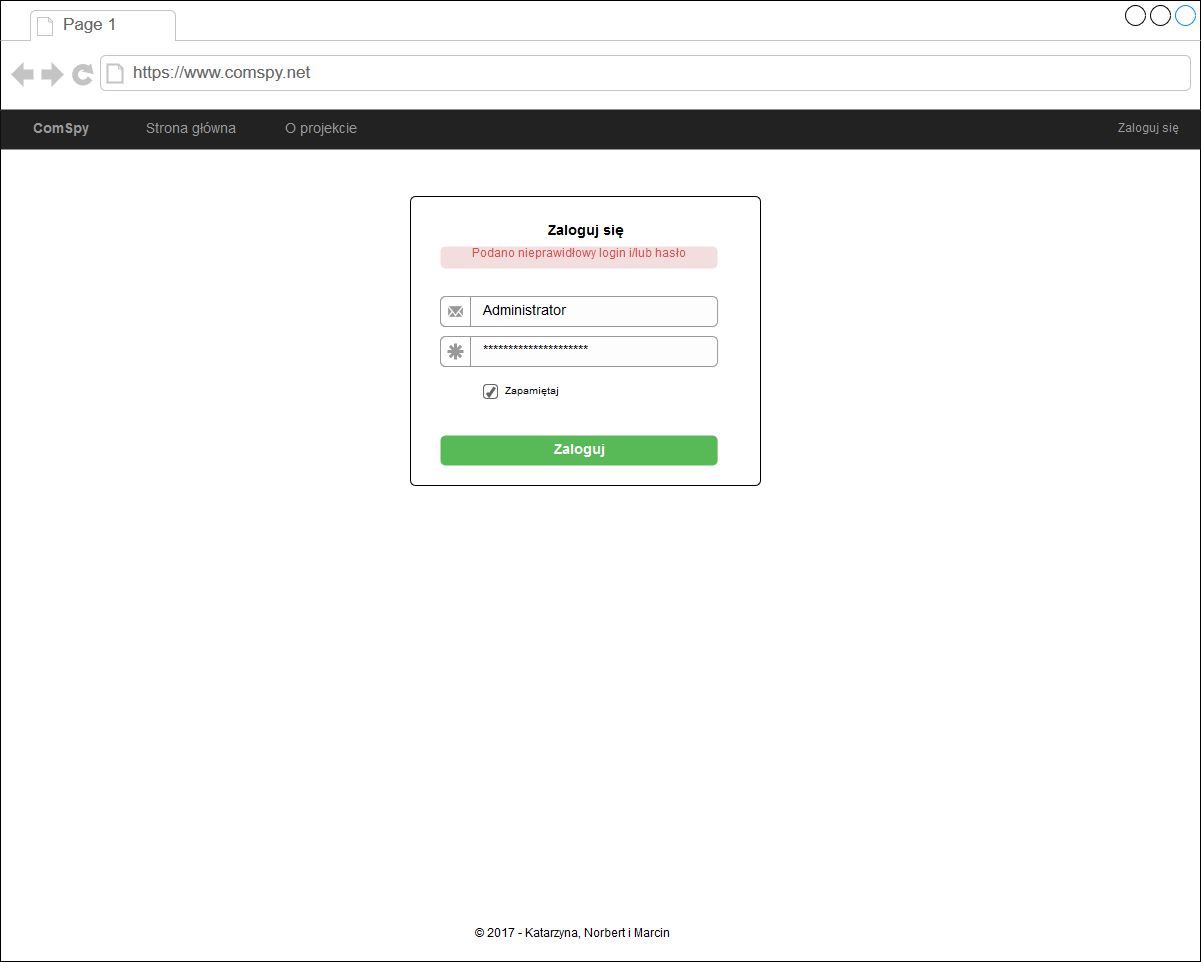
\includegraphics[height=12cm,width=15cm]{interfejs_zaloguj}
    \caption{Projekt strony logowania}
    \label{fig:my_label}
\end{figure}

\newpage
Rysunek nr 10 przedstawia projekt strony poglądu głównego, który jest widoczny dla użytkowników zalogowanych (oraz Administratorów). Widać tutaj podglądy wybranych przez użytkownika grup stanowisk oraz okienka z ostrzeżeniami związanymi z naruszeniem listy dozwolonych stron do przeglądania (blacklist)
\begin{figure} [!ht]
    \centering
    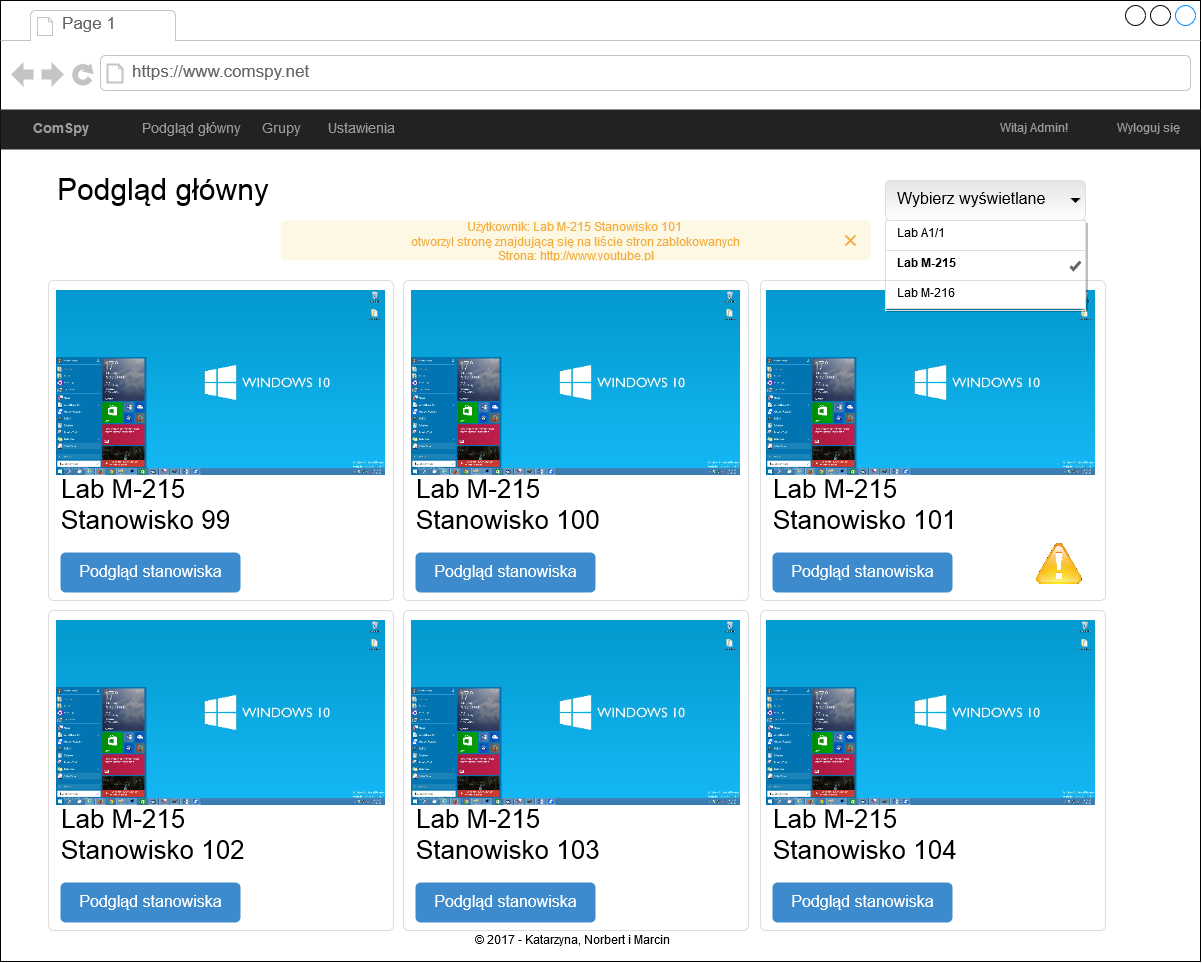
\includegraphics[height=12cm,width=15cm]{interfejs_podglad_glowny}
    \caption{Projekt strony - podgląd główny (dostępny po zalogowaniu)}
    \label{fig:my_label}
\end{figure}


\newpage
Rysunek nr 11 przedstawia projekt podglądu szczegółowego jednego stanowiska. Tutaj oprócz samego zrzutu ekranu wyświetlane są informacje o uruchomionych procesach, otwartych stronach internetowych oraz podstawowe dane konfiguracyjne.
\begin{figure} [!ht]
    \centering
    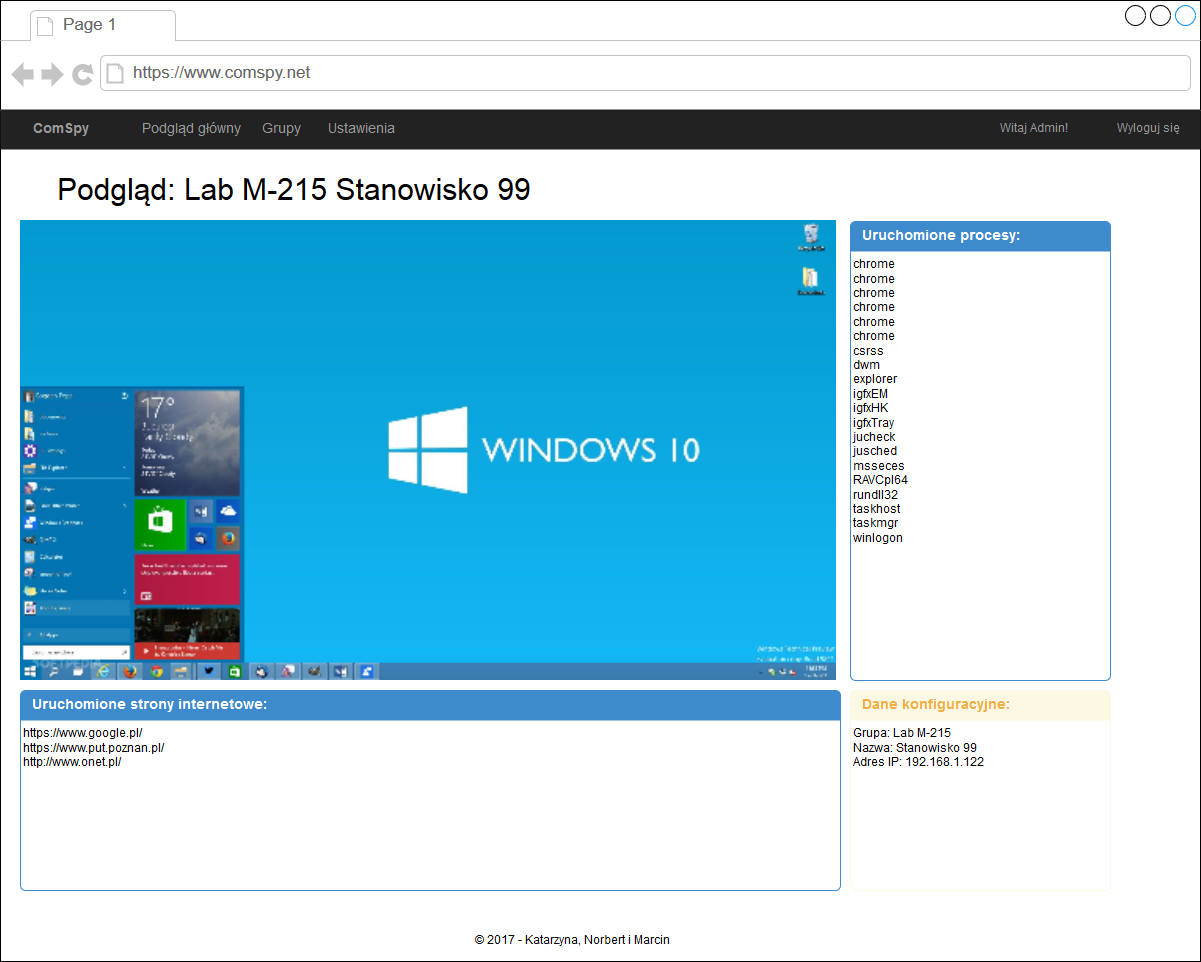
\includegraphics[height=12cm,width=15cm]{interfejs_podglad_stanowiska}
    \caption{Projekt strony - podgląd stanowiska (dostępny po zalogowaniu)}
    \label{fig:my_label}
\end{figure}


\newpage
Rysunek nr 12 przedstawia zarządzanie grupami oraz stanowiskami w ramach jednej z nich. Ten widok dostępny jest tylko dla administratorów.
\begin{figure} [!ht]
    \centering
    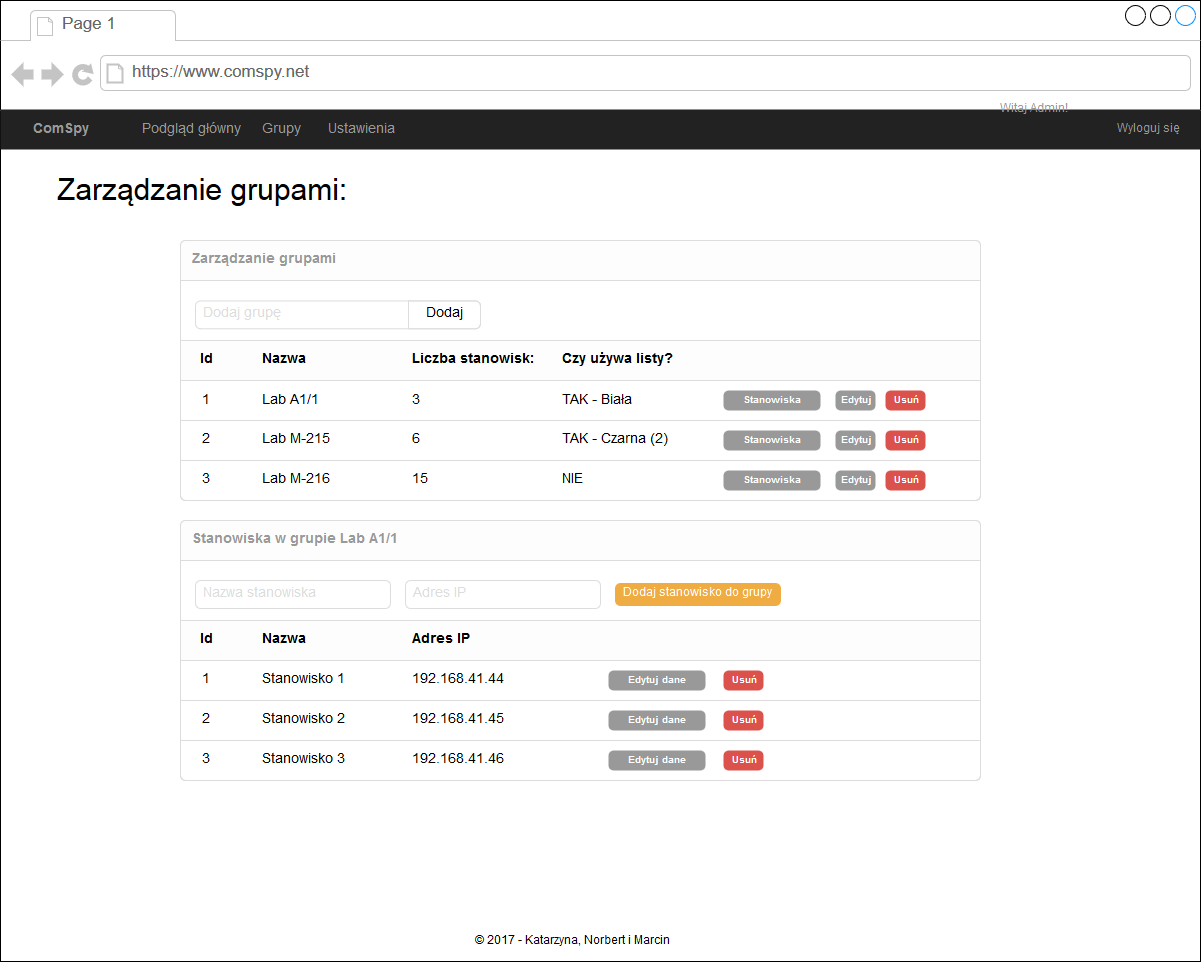
\includegraphics[height=12cm,width=15cm]{interfejs_grupy}
    \caption{Projekt strony - zarządzanie grupami i stanowiskami (dostępny po zalogowaniu)}
    \label{fig:my_label}
\end{figure}


\newpage
Rysunek nr 13 przestawia panele dotyczące zarządzania użytkownikami oraz blacklistą.
\begin{figure} [!ht]
    \centering
    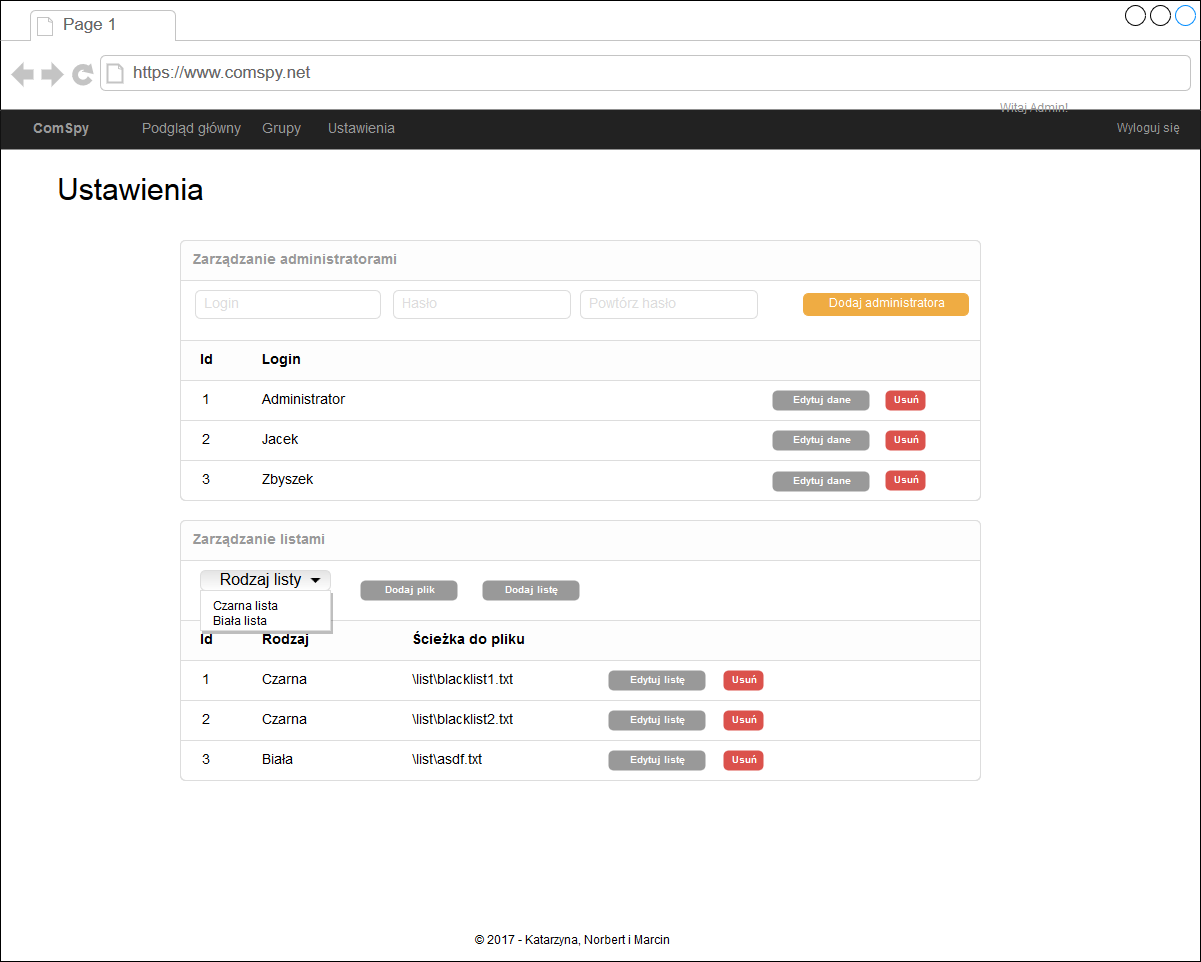
\includegraphics[height=12cm,width=15cm]{interfejs_ustawienia}
    \caption{Projekt strony - ustawienia (dostępny po zalogowaniu)}
    \label{fig:my_label}
\end{figure}


\newpage

\subsection{Aplikacja kliencka}
Ostatni szkic przedstawia program klienta, na którym widać niepodłączonego jeszcze klienta do serwera. Oprócz samego statusu połączenia widać adres IP serwera oraz identyfikator stanowiska. Widać także przyciski Podgląd, która przeniesie do okna, w którym można podejrzeć chwilowy stan tego, co jest następnie przesyłane do serwera. Po kliknięciu w przycisk Administrator natomiast można natomiast w przyszłości zaimplementować podstawowy panel administracyjny lub inne funkcje, które dostępne będą tylko dla administratora systemu.


\begin{figure} [!ht]
    \centering
    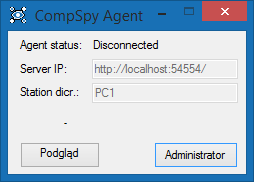
\includegraphics[height=6cm,width=8cm]{interfejs_agent}
    \caption{Projekt strony - ustawienia (dostępny po zalogowaniu)}
    \label{fig:my_label}
\end{figure}
    \section{Bezpieczeństwo}

Podczas tworzenia projektu postarano się, aby zapewnić w bezpieczeństwo pod wieloma aspektami. Poniżej przedstawiono najważniejsze z nich oraz sposoby ich zapewnienia.
\newline

Hasła przechowywane w bazie danych nie są przechowywane w formie jawnej, lecz w postaci heksadecymalnego skrótu powstałego przy użyciu funkcji skrótu SHA-256.  Podczas wpisywania samego hasła w polu tekstowym, hasło jest zakropkowane.


W serwisie internetowym zapewniono, aby dostęp do poszczególnych funkcjonalności był możliwy tylko dla osób z odpowiednimi uprawnieniami (np. podgląd możliwy tylko dla użytkowników zalogowanych). Same widoki nie powinny być również dostępne po wpisaniu adresu w pasku adresu przeglądarki. 


Innym rodzajem bezpieczeństwa jest zabezpieczenie przed zbędnym przesyłaniem pakietów i zmniejszeniu przepustowości sieci. Polega to na tym, że gdy żaden użytkownik w serwisie internetowym nie podgląda stanowisk, to stanowiska nie przesyłają w tym czasie dużych pakietów ze zrzutami ekranów, listą włączonych procesów oraz listą otwartych kart w przeglądarkach.


Kolejnym zabezpieczeniem jest rozdzielenie użytkowników na użytkownika zalogowanego oraz administratora. Dzięki temu użytkownik ma dostęp do poglądu, ale nie może usunąć ani zarządzać grupami oraz stanowiskami. Uprawnienia do ich dodawania, edycji i usuwania ma tylko konto z uprawnieniami administratora.
    \lstdefinestyle{sharpc}{language=[Sharp]C, frame=lr, rulecolor=\color{blue!80!black}}


\section{Napotkane problemy}

W poniższym rozdziale opisane zostały najważniejsze problemy z jakimi spotkała się grupa projektowa w trakcie projektowania oraz już samej implementacji.
\newline

\subsection{Tworzenie zrzutów ekranu oraz pobieranie listy procesów aktywnych}
Pierwszym problemem jaki wystąpił, było tworzenie zrzutów ekranu oraz listy procesów na komputerze klienta. To był najłatwiejszy problem z jakim spotkała się grupa. Aby rozwiązać problem wystarczyło wykorzystać dostępne w środowisku .NET funkcje. Samo zrobienie zrzutu to tak na prawdę wykorzystanie dokładnie jednej funkcji.

\newline
\begin{lstlisting}[frame=single,captionpos=b,
    caption={Fragment kodu odpowiedzialny za tworzenie zrzutów ekranu},
    label={lst:kod1},
    style=sharpc]
bmp = new Bitmap(Screen.PrimaryScreen.Bounds.Width,
    Screen.PrimaryScreen.Bounds.Height,
    System.Drawing.Imaging.PixelFormat.Format32bppRgb);
    zrzut = Graphics.FromImage(bmp);
    zrzut.CopyFromScreen(0, 0, 0, 0,
        Screen.PrimaryScreen.Bounds.Size,
        CopyPixelOperation.SourceCopy);
\end{lstlisting}

\begin{lstlisting}[frame=single,captionpos=b,
    caption={Fragment kodu odpowiedzialny za pobranie listy aktywnych procesów},
    label={lst:kod1},
    style=sharpc]
public Process[] listaProcesow;
listaProcesow = Process.GetProcesses();
\end{lstlisting}


\subsection{Uzyskanie adresów kart w przeglądarkach internetowych}
Drugim problemem było pytanie, jak uzyskać adresy stron internetowych. Samo wyświetlenie tytułów było łatwe, ponieważ wykorzystano podobnie jak w poprzednim problemie dostępne funkcje w środowisku. NET. Samo zdobycie tytułów otwartych okien zostało pokazane na przykładzie przeglądarki Chrome na listingu nr 3.
\newline
\begin{lstlisting}[frame=single,captionpos=b,
    caption={Fragment kodu odpowiedzialny za pobranie tytułu otwartej strony w przeglądarce Chrome.},
    label={lst:kod1},
    style=sharpc]
foreach (var p in listaProcesow)
{
    if (Convert.ToString(p.ProcessName) == "chrome")
    {
        if (p.MainWindowTitle != "" ||
            p.MainWindowTitle == " ")
        {
            listaStron.Add("[chrome]");
            listaStron.Add ("Title: " + 
                p.MainWindowTitle);
        }
    }
}
\end{lstlisting}

Powyższy sposób został użyty do pobrania tytułów z przeglądarek: Chrome, Opera, Internet Explorer oraz Microsoft Edge (działanie tej ostatniej nie zostało potwierdzone, ze względu na brak testów w systemie Windows 10). Dzięki wykorzystaniu biblioteki NDde udało się pobrać nie tylko tytuł, ale także adres strony internetowej otwartej w przeglądarce Mozilla Firefox. Ze względu na ograniczony czas pracy nad systemem i wystąpieniem tak wielu problemów, obecnie nie działa to dla innych przeglądarek.

\newline



\begin{lstlisting}[frame=single,captionpos=b,
caption                 ={Fragment kodu odpowiedzialny za pobranie adresu URL oraz tytułu otwartej strony w przeglądarce Mozilla Firefox},
label                   ={lst:kod1},
style                   =sharpc]

using NDde.Client;

public void getURLfirefox()
{
    try
    {
        DdeClient dde = new DdeClient("firefox",
            "WWW_GetWindowInfo");
        dde.Connect();
        string url = dde.Request("URL", int.MaxValue);
        string[] urls = url.Split(new string[] 
            { ",", "\"" }, 
            StringSplitOptions.RemoveEmptyEntries);
        dde.Disconnect();
        
        listaStron.Add("[firefox]");
        listaStron.Add("URL: " + urls[0]);
        listaStron.Add("Title: " + urls[1]);
    }
    catch {}
}
\end{lstlisting}

\subsection{Konwersja zrzutu ekranu}

Następnym problemem, jaki napotkała grupa projektowa, było to to w jaki sposób przesłać zrzut ekranu. Okazało się że najlepszym sposobem będzie konwersja zdjęcia (już po zmianie formatu oraz rozmiaru w zależności od tego w jakiej jakości żąda serwer) do formatu tekstowego za pomocą konwersji do typu Base64. 

\newline
\begin{lstlisting}[frame=single,captionpos=b,
    caption={Fragment kodu odpowiedzialny za konwersję obrazu.},
    label={lst:kod1},
    style=sharpc]
public String getImageBase64(Bitmap img)
{
    Graphics g = Graphics.FromImage(img);
    
    System.IO.MemoryStream stream = 
        new System.IO.MemoryStream();
    img.Save(stream, 
        System.Drawing.Imaging.ImageFormat.Bmp);
    byte[] imageBytes = stream.ToArray();
    
    return Convert.ToBase64String(imageBytes);       
}
\end{lstlisting}

\subsection{Wykorzystanie SignalR}
Po konwersji następuje już budowa samego komunikatu. Następnie następuje serializacja komunikatu i wysłanie go do serwera. Ale nie jest to takie łatwe, ponieważ problemem okazała się kwestia, aby nie przesyłać niepotrzebnie pakietów, gdy żaden użytkownik nie korzysta z serwisu internetowego i nie podgląda stanowisk. Rozwiązaniem okazało się wykorzystanie biblioteki SignalR. Pierwszym listingiem, który został ukazany jest sama konfiguracja uchwytu serwera, który zawiera w sobie hub do obsługi połączenia.

\newpage
\newline
\begin{lstlisting}[frame=single,captionpos=b,
    caption={Fragment kodu - konstruktor klasy ServerHandler},
    label={lst:kod1},
    style=sharpc]
public ServerHandler
    (string hubAddr, ApplicationForm appForm)
 {
    this.hubAddr = hubAddr;
    this.appForm = appForm;
    
    hubConnection = new HubConnection(hubAddr);
    
    computerHub = 
        hubConnection.CreateHubProxy("ComputerHub");
        
    ConfigureRPCHandlers();
}
\end{lstlisting}

Ważnym elementem wykorzystania tej klasy jest metoda ustanawiająca połączenie. Podczas nawiazywania tego połączenia jest przesyłana informacja o identyfikatorze stanowiska oraz sekret.


\begin{lstlisting}[frame=single,captionpos=b,
    caption={Fragment kodu metody nawiązującej połączenie},
    label={lst:kod1},
    style=sharpc]
private void EstablishConnection()
{
    var parameters = new Dictionary<string, string>
    {
        { "stationId", ConfigurationManager.AppSettings
                ["stationDiscr"]},
                
        { "secret", ConfigurationManager.AppSettings
                ["secret"] }
    };
    
    computerHub.Invoke("Connect", 
        ConfigurationManager.AppSettings
        ["stationDiscr"]);
}
\end{lstlisting}

\newpage
Poniżej przedstawiono sposób wysyłania komunikatu dla żądania rozpoczęcia transmisji niskiej jakości. Fragment pochodzi z metody odpowiedzialnej za konfigurację uchwytu RPC.

\begin{lstlisting}[frame=single,captionpos=b,
    caption={Fragment kodu przedstawiający wysyłanie komunikatu dla rozpoczęcia transmisji niskiej jakości.},
    label={lst:kod1},
    style=sharpc]
computerHub.On("StartLowQualityTransmission", () =>
{
    Spy spy = new Spy();
    spy.Aktualizacja();
    var data = spy.serializacja(false);
    computerHub.Invoke("ReceiveData", data);
});
\end{lstlisting}







    \section{Komunikacja}

W poniższym rozdziale zostanie w krótki sposób opisany sposób komunikacji pomiędzy poszczególnymi częściami systemu. Wyróżniamy dwa rodzaje komunikacji: pierwszy to komunikacja użytkownika serwisu internetowego z serwerem tego systemu, drugi to natomiast komunikacja klientów z serwerem. 

\vspace{0.5cm}

Komunikacja pomiędzy serwisem internetowym i jej klientem odbywa się w standardowy sposób dla technologii ASP.NET. Postawiony system na serwerze IIS(Internet Information Services) zawiera pliki napisane z wykorzystaniem HTML, JavaScript oraz C#. Komunikacja odbywa się za pośrednictwem protokołu HTTP.
\vspace{0.5cm}

Komunikacja pomiędzy klientami a serwisem internetowym wykorzystuje bibliotekę SignalR. Wykorzystanie jej jest opisane w rozdziale 12 zatytułowanym "Napotkane problemy". Poniżej natomiast przedstawiona jest budowa komunikatu, który jest wysyłany od klienta do serwera. 

\vspace{0.5cm}
\begin{lstlisting}[frame=single,captionpos=b,
    caption={Fragment kodu przedstawiający budowę klasy Komunikat},
    label={lst:kod1},
    style=sharpc]
[DataContract]
public class Komunikat
{
    [DataMember]
    public String image { get; set; }
    [DataMember]
    public List<String> listaProcesow { get; set; }
    [DataMember]
    public List<String> listaStron { get; set; }

    public Komunikat(String img, Process[] procesy,
        List<String> strony) {
        image = img;
        listaProcesow = new List<String>();
        listaStron = new List<String>();
        foreach (var p in procesy)
            listaProcesow.Add(p.ProcessName);
        foreach (var s in strony)
            listaStron.Add(s);
    }
}
\end{lstlisting}

Podczas tworzenia powyższego komunikatu wprowadzane są
 dane aktualne z listy procesów, listy stron oraz tworzony jest zrzut ekranu. Po tym procesie komunikat jest serializowany. Format samego komunikatu, który jest już przesyłany do serwera jest w formacie XML. W kolejnym listingu przedstawiony jest przykład takiego pliku.
 
 \begin{lstlisting}[frame=single,captionpos=b,
    caption={Przykładowy komunikat przesyłany do serwera w formacie XML},
    label={lst:kod1},
    language=XML]
<Spy.Komunikat 
    xmlns="http://schemas.datacontract.org/2004/07/
        CompSpyAgent"
   xmlns:i="http://www.w3.org/2001/XMLSchema-instance">
  <image>
    ...
    zrzut ekranu jako base64
    ...
  </image>
  <listaProcesow xmlns:a="http://schemas.microsoft.com/2003/
    10/Serialization/Arrays">
    <a:string>svchost</a:string>
    <a:string>notepad++</a:string>
    <a:string>isesrv</a:string>
    <a:string>services</a:string>
    <a:string>winlogon</a:string>
    <a:string>chrome</a:string>
    <a:string>conhost</a:string>
    <a:string>explorer</a:string>
  </listaProcesow>
  <listaStron xmlns:a="http://schemas.microsoft.com/
    2003/10/Serialization/Arrays">
    <a:string>[firefox]</a:string>
    <a:string>URL: https://www.google.pl</a:string>
    <a:string>Title: Google</a:string>
    <a:string>[chrome]</a:string>
    <a:string>Title: Onet.pl - Google Chrome</a:string>
  </listaStron>
</Spy.Komunikat>
\end{lstlisting}
    \section{Testy}

W poniższym rozdziale przedstawione zostaną testy systemu. Zostały one wykonane na różnych etapach prac. Część widoków została utworzona specjalnie do tego, aby przetestować różne funkcjonalności systemu, a nie znajdą się w finalnej wersji produktu.

\newline \newline
Do pierwszych testów tworzenia zrzutów ekranu oraz pobierania listy aktywnych procesów napisano aplikację Windows Form, która po kliknięciu na przycisk "Zrzut" wyświetlany jest zrzut ekranu oraz lista procesów.

\begin{figure} [!ht]
    \centering
    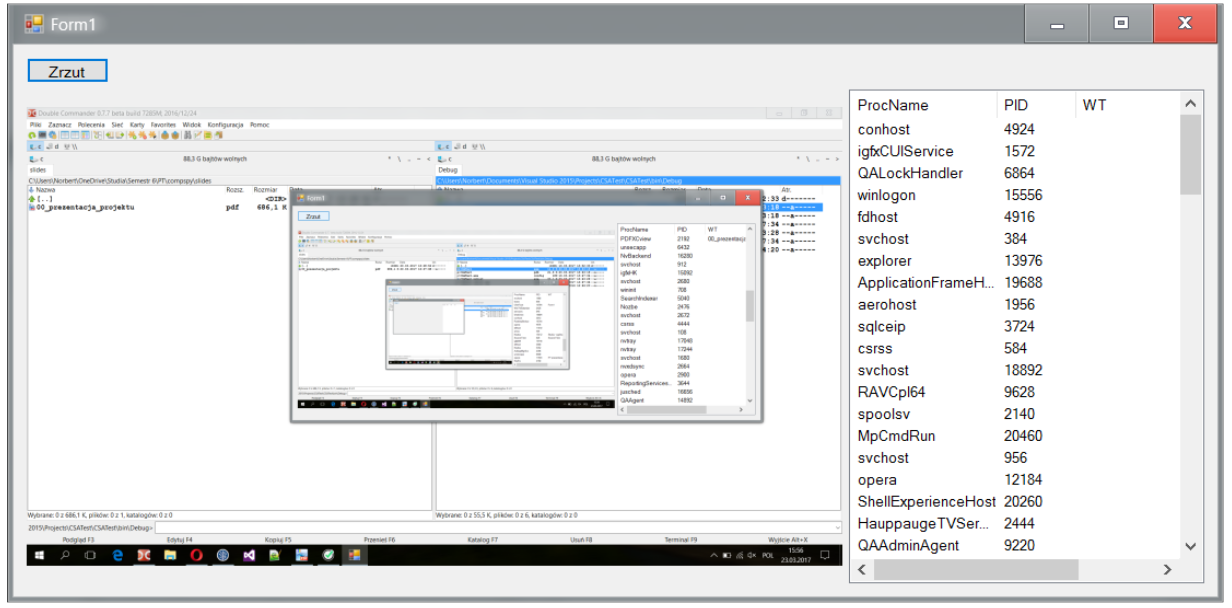
\includegraphics[height=9cm,width=16cm]{comspy_testy1}
    \caption{Testowanie funkcjonalności tworzenia zrzutów ekranu oraz pobierania listy aktywnych procesów.}
    \label{fig:my_label}
\end{figure}

\newpage
Gdy już udało się wybrać odpowiednie rozwiązanie postanowiono zbudować okno do podglądu w aplikacji klienta, aby można było sprawdzić działanie jeszcze przed połączeniem się do serwera i wysłaniem komunikatu. W tej wersji (w porównaniu do poprzedniego programu) działa również podgląd adresów i tytułów otwartych kart w przeglądarkach, a także zmiana jakości obrazu (niska i wysoka jakość). We wcześniejszej wersji korzystano także z funkcjonalności zegara do aktualizacji co określony czas.


\begin{figure} [!ht]
    \centering
    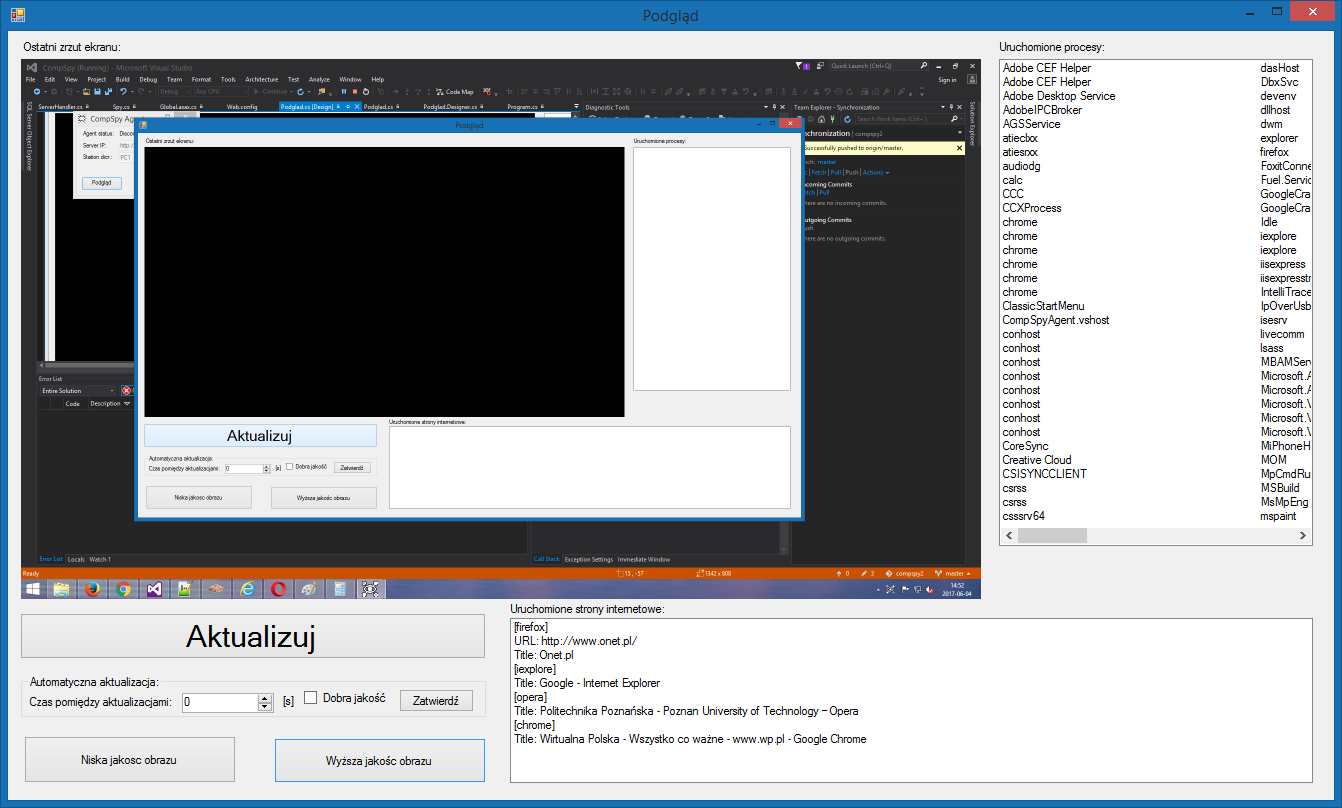
\includegraphics[height=9cm,width=16cm]{comspy_testy3}
    \caption{Widok Podgląd w aplikacji klienta}
    \label{fig:my_label}
\end{figure}

\newpage
Gdy udało się połączyć aplikację klienta i serwer z pomocą biblioteki SignalR zaczęto także testować uruchamianie z poziomu strony metod wywoływanych u klienta. Rysunek nr 17 przedstawia możliwe przykładowe wykorzystanie takiego połączenia.

\begin{figure} [!ht]
    \centering
    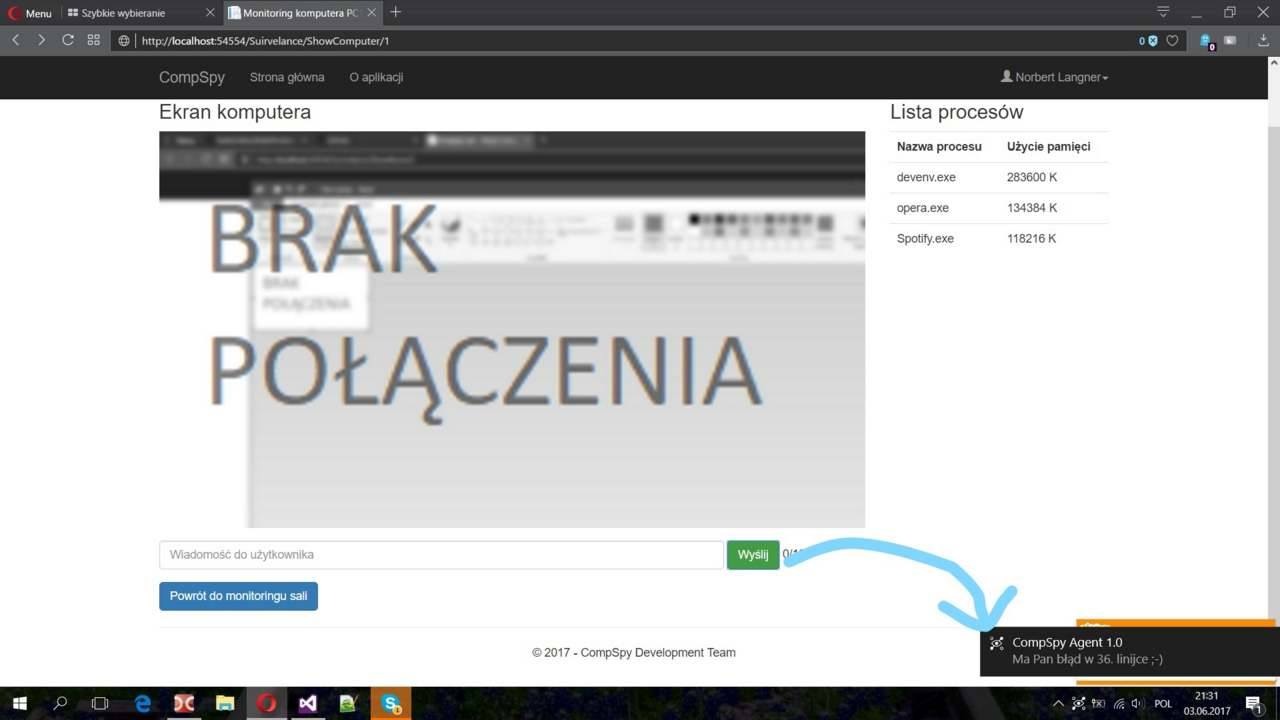
\includegraphics[height=9cm,width=16cm]{comspy_testy4}
    \caption{Testowanie funkcjonalności SignalR za pomocą wysyłania wiadomości do aplikacji klienta.}
    \label{fig:my_label}
\end{figure}

\newpage
Ostatni przedstawiony test miał już miejsce po wysłaniu poprawnego komunikatu przez klienta do serwera. Za pomocą narzędzi deweloperskich dostępnych w przeglądarce Opera sprawdzono otrzymany komunikat.

\begin{figure} [!ht]
    \centering
    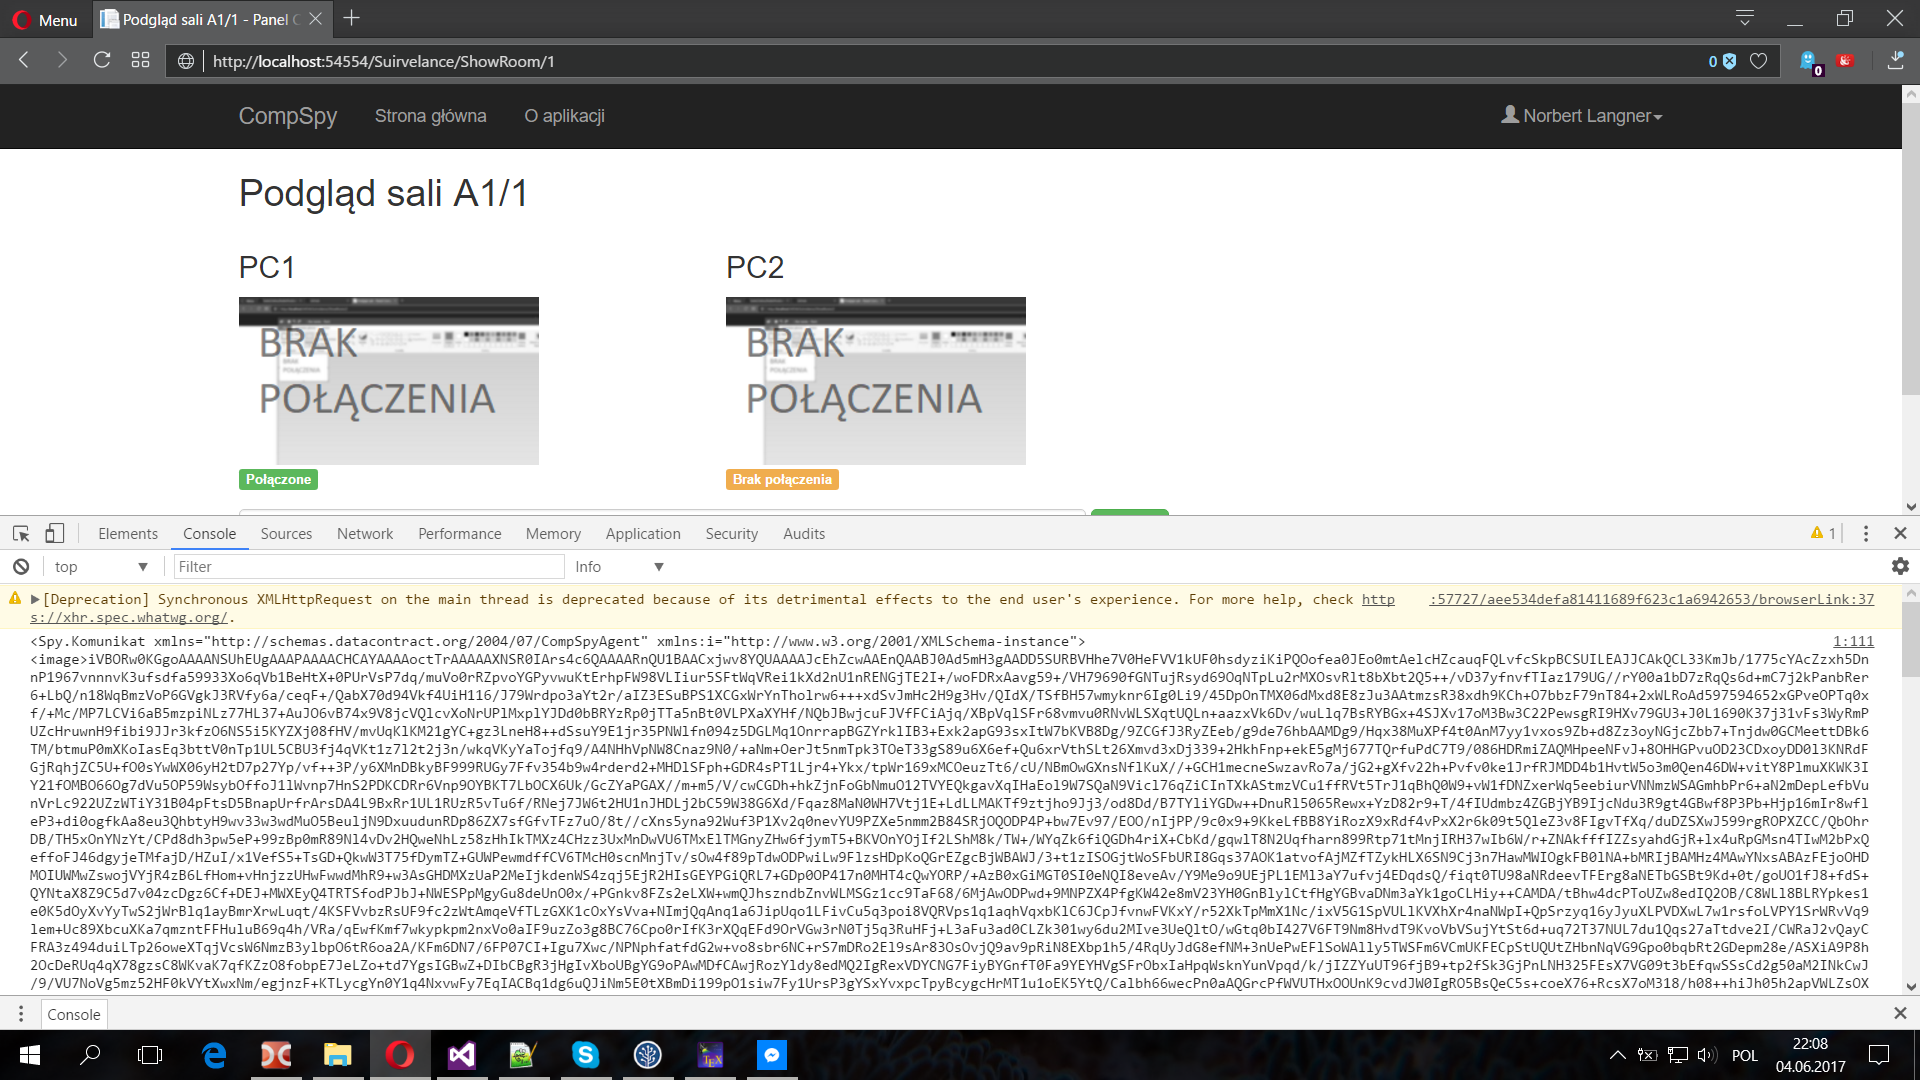
\includegraphics[height=9cm,width=16cm]{comspy_testy9}
    \caption{Podgląd komunikatu otrzymanego od klienta}
    \label{fig:my_label}
\end{figure}
    \section{Podział prac}

W poniższej tabeli nr 5 przedstawiono podział prac pomiędzy osoby należące do grupy projektowej.

\begin{table}[!ht]
\caption{\label{tab:widgets}Podział prac}
\begin{tabular}{| m{8cm} | m{1.6cm} | m{1.6cm} | m{1.6cm} |} 

\hline
Część projektu & Norbert & Kasia & Marcin \\ \hline

Tworzenie dokumentacji & X  & X &  X \\ \hline

Utworzenie projektu bazy danych & X  & X &  X \\ \hline

Utworzenie diagramu przypadków użycia &   & X &   \\ \hline

Utworzenie diagramów klas &   &  &  X \\ \hline

Rozwiązanie problemu tworzenia zrzutów ekranu & X  &  &   \\ \hline
Rozwiązanie problemu tworzenia listy aktywnych procesów &   & X &   \\ \hline

Rozwiązanie problemu pobierania adresów otwartych stron internetowych &   &  &  X \\ \hline

Implementacja programu klienta & X  &  &  X \\ \hline
Implementacja serwisu internetowego i serwera & X  & X &   \\ \hline








\end{tabular}
\end{table}
    \section{Możliwości rozwoju}

Poniższy rozdział przedstawia możliwe kierunki rozwoju dla systemu. Podzielono te kierunki na dwie kategorie: rozszerzające lub dodające nowe funkcjonalności oraz zwiększające przyjazność obsługi dla użytkownika. Dodatkowo można wspomnieć o możliwości optymalizacji wykorzystania zasobów komputera oraz wykorzystania łącza sieciowego. 

\subsection{Funkcjonalności}
W tym podrozdziale skupiono się na możliwościach rozwoju działających już funkcjonalności oraz takim, które można dodać do systemu.

    Pierwszą rzeczą, jaką można utworzyć jest to utworzenie aplikacji klienckiej dla systemu operacyjnego Linux. Dzięki takiemu rozwiązaniu, system będzie wspierał sale, w których korzysta się z innego systemu operacyjnego niż Windows.
    
    Drugim rozwiązaniem może być połączenie systemu z innymi, w celu np. identyfikacji studenta/ucznia i powiązaniem go ze zdarzeniami związanymi w nim. W takim przypadku można np. wykorzystać do sprawdzenia w późniejszym terminie historii ostrzeżeń studenta bez pamiętania jego stanowiska, przy którym siedział. 
    
    
    Kolejnym rozszerzeniem mogłoby być dodanie większej ilości informacji o procesach i wykorzystaniu komputera przez użytkownika. Może to być informacja u procencie wykorzystania procesora, ilości wykorzystywanej pamięci oraz łącza internetowego. To ostatnie może być także użyte do prowadzenia statystyk związanych z wykorzystywaniem systemu CompSpy w salach laboratoryjnych.
    
    
    Dosyć ważnym rozszerzeniem byłoby utworzenie rozszerzeń do przeglądarek internetowych wykorzystywanych w salach laboratoryjnych, aby była możliwość pobrania wszystkich otwartych kart w przeglądarkach, a nie tylko jednej aktualnie otwartej.
    
\newpage
\subsection{Przyjazność dla użytkownika}
W tej sekcji postanowiono opisać możliwości rozwoju związane z samym interfejsem użytkownika i funkcjonalnościami, które maj poprawić wygodę korzystania z systemu.


Jedną z możliwości polepszenia interfejsu użytkownika jest stworzenie aplikacji okienkowej, która będzie służyć tylko do podglądu stanowisk. Można by taką aplikację udostępniać w danych salach laboratoryjnych na np. jednym stanowisku komputerowym, gdzie dostęp do podglądu nie wymagałby konta w systemie ale byłby powiązany tylko z daną salą. Dzięki takiemu rozwiązaniu nauczyciele nie musieliby się logować do systemu, lecz taki program mógłby działać od początku uruchomienia systemu operacyjnego i w każdym momencie mogliby do niego przejść.

Drugim rozszerzeniem, które zostało uznane przez grupę za ciekawe jest utworzenie wielu wersji językowych systemu, szczególnie wersji angielskiej. Dzięki takiemu rozwiązaniu nauczyciele, którzy są np. z zagranicznych uczelni mogliby też korzystać.
\end{document}
